\subsubsection{Generalized recirculation}
\label{sec:models-generec} 

\paragraph{Introduction.} 
The \emph{Generalized recirculation algorithm}, or \emph{GeneRec}, was developed by \citet{o1996bio}. It's a supervised algorithm which in comparison with Backpropagation \ref{sec:models-bp} is argued to be a more biologically plausible model as error is computed locally as a difference between activations \citep{o1998six, o2001generalization, da2011advances, schneider2009application}. In summary, GeneRec is a combination of CHL \ref{sec:models-chl} and the Recirculation algorithm \ref{sec:models-recirc}. It overcomes limitations of the Recirculation algorithm to be an encoder by having a three layer network. For the error computation a backward weight matrix from output layer to hidden layer is used and the learning rule is derived from the CHL learning rule~\ref{eq:models-chl-learning-rule}. It could be proven that GeneRec, as Backpropagation, could learn arbitrary input--output mappings \citep{o1996bio}. 

\paragraph{Learning rule.} 
\label{sec:models-generec-learning-rule} 
GeneRec uses three weight matrices $W^{IH}$, $W^{HO}$ and $W^{OH}$ for the input--hidden, hidden--output and output--hidden weights. It also has the \quotes{-} and \quotes{+} phases as CHL with same meaning, i.e. in the \emph{minus} phase only the input vector is clamped and in the \emph{plus} phase both input and target vectors are clamped as seen on table~\ref{tab:models-generec}. Generec uses the non--symmetric version of the CHL rule for all three weight matrices: 
\begin{equation}
  \label{eq:models-generec-learning-rule}
  \Delta w_{ij} = \lambda a^{-}_i(a^{+}_j - a^{-}_j)
\end{equation}
where $a^{-}_p$ denotes the presynaptic and $a^{-}_q$ denotes the postsynaptic unit activation in minus phase, $a^{+}_p$ is the presynaptic activation from plus phase and $\lambda$ denotes the learning rate. So for example when updating $W^{HI}$ then $a^{-}_i = h^{-}_i$, $a^{-}_j = o^{-}_j$ and $a^{+}_j = t_k$. 

\paragraph{Activation.} 
\label{sec:models-generec-activation} 
The main difference between CHL and GeneRec is that GeneRec has layers and it's based more on Recurrent neural networks than on the Hopfield networks. Therefore, as shown in table~\ref{tab:models-generec}, we can compute the activations sequentially. 
\begin{table}
  \centering
  \begin{tabular}{|cccc|}
    \hline
    Layer & Phase & Net Input & Activation\\
    \hline
    Input (s)    & $-$ & - & $s_i$ = \mbox{stimulus input} \\
    \hline
    Hidden (h)   & $-$ & \hspace{0.3cm}$\eta^{-}_j = \sum_i w_{ij}^{IH}s_i + \sum_k w_{kj}^{OH}o^{-}_k$\hspace{0.3cm} &
    $h^{-}_j = \sigma(\eta^{-}_j)$\hspace{0.3cm}\\
          &  +  & $\eta^{+}_j = \sum_{i}w_{ij}^{IH}s_i + \sum_k w_{kj}^{OH}o^{+}_k$ & $h^{+}_{j} = \sigma(\eta^{+}_j)$ \\
    \hline
    Output (o) & $-$ & $\eta^{-}_k = \sum_j w_{jk}^{HO}h_j$ & $o^{-}_k = \sigma(\eta^{-}_k)$\\
           &  +  & - & $o^{+}_k$ = \mbox{target output} \\
    \hline
  \end{tabular}
  \caption{Equilibrium network variables in GeneRec model \citet{o1996bio}. We can see the inspiration from the Recirculation algorithm \ref{sec:models-recirc} and a correspondence between $T$ and GeneRec phases. In particular $s^{-} \approx T=0$, $h^{-} \approx T=1$, $o^{-} \approx T=2$ and $h^{+}$ corresponds to $T=3$. The activation flow is depicted on figure~\ref{fig:models-generec-phase}.}
  \label{tab:models-generec}
\end{table}
In case of the \emph{plus} phase only the hidden activations are necessary to compute what could be achieved by computing $\phi(\eta_i)$. In case of the \emph{minus} phase where only inputs are clamped it's necessary to find an \emph{equilibrium} activation state for which the equations~\ref{tab:models-generec} hold. As dicussed in recurrent networks~\ref{sec:theory-recurrent} there are several approaches. In our implementation~\ref{sec:appendix-impl-generec} we choose the \emph{iterative method} with following rules for computing activations $a_i$: 
\begin{align}
  \label{eq:models-generec-activation}
  a_i(0) = \left\{
	\begin{array}{ll}
		s_i & \mbox{if } i \in \mbox{input} \nonumber \\
		0 & \mbox{otherwise} \nonumber 
	\end{array}
\right. \\
  a_i(t+1) = \left\{
	\begin{array}{ll}
		s_i & \mbox{if } i \in \mbox{input} \nonumber \\
		\phi(\sum_j w_{ji}a_j(t)) & \mbox{otherwise} \nonumber 
	\end{array}
\right. \\
\end{align} 
where $a_i(t)$ is the activation of $i$--th unit in discrete time $t$. The rules~\ref{eq:models-generec-activation} while are iterated while $|a_i(t+1) a_i(t)| > \epsilon$ for some unit $i$. This method is further discussed in \ref{sec:generec-fluctuation} and \citep{orru2008sabio}.

\begin{figure}[h]
  \centering
  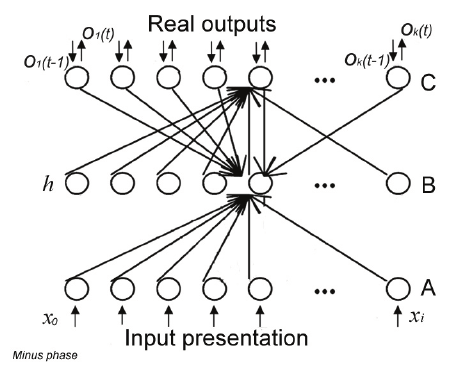
\includegraphics[width=0.4\textwidth]{img/generec_minus_phase.png}
  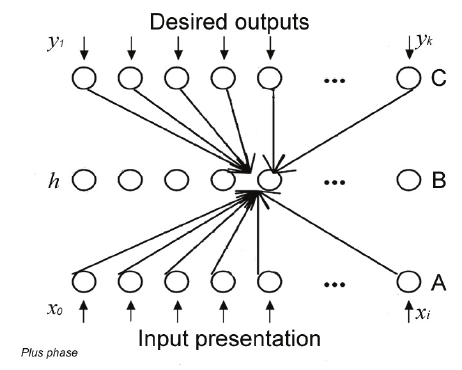
\includegraphics[width=0.4\textwidth]{img/generec_plus_phase.png}
  \caption{Depicting the minus and plus phases of GeneRec \citet{orru2008sabio}. The activation equations are defined in table~\ref{tab:models-generec}. TODO redraw and merge} 
  \label{fig:models-generec-phase}
\end{figure}

\paragraph{Modifications.}
\label{sec:models-generec-modifications} 
It's important to note that \citet{o1996bio} proved that GeneRec converges if the learning rule~\ref{eq:models-generec-learning-rule} is a valid approximation to the error derivate and the weights beeing symmetric, i.e. $W^{HO} = W^{OH^{T}}$. \citet{o1996bio} based on CHL and the midpoint method for fradient computation \citep{press1990numerical} proposed two more learning rules for GeneRec: 
\begin{equation}
  \label{eq:models-generec-learning-rule-mid}
  \frac{1}{\lambda} \Delta w_{ij} =  \frac{1}{2}(a^{-}_i + a^{+}_i)(a^{+}_j - a^{-}_j)
\end{equation}
\begin{equation}
  \label{eq:models-generec-learning-rule-sym}
  \frac{1}{\lambda} \Delta w_{ij} =  (a^{+}_j a^{-}_i - a^{-}_j a^{+}_i) - 2a^{-}_j a^{-}_i
\end{equation}
where~\ref{eq:models-generec-learning-rule-mid} is called the \emph{midpoint learning rule} and~\ref{eq:models-generec-learning-rule-sym} is called the \emph{symmetric learning rule} which aims to preserve weight symmetry. By combining rules ref{eq:models-generec-learning-rule-mid} and \ref{eq:models-generec-learning-rule-sym} we get the following rule: 
\begin{equation}
  \label{eq:models-generec-learning-rule-chl}
  \frac{1}{\lambda} \Delta w_{ij} =  (a^{+}_i a^{+}_j) - (a^{-}_i a^{-}_j)
\end{equation}
which is indeed the CHL learning rule~\ref{eq:models-chl-learning-rule}. Thus we see that GeneRec is closely related to CHL. 

Note that we encountered some missing details in \citet{o1996bio} about how to implement the GeneRec algorithm which are further discussed in \ref{sec:appendix-impl-generec}.
